\section{Bau eines Keplerschen Fernrohrs}

\begin{figure}
    \centering
    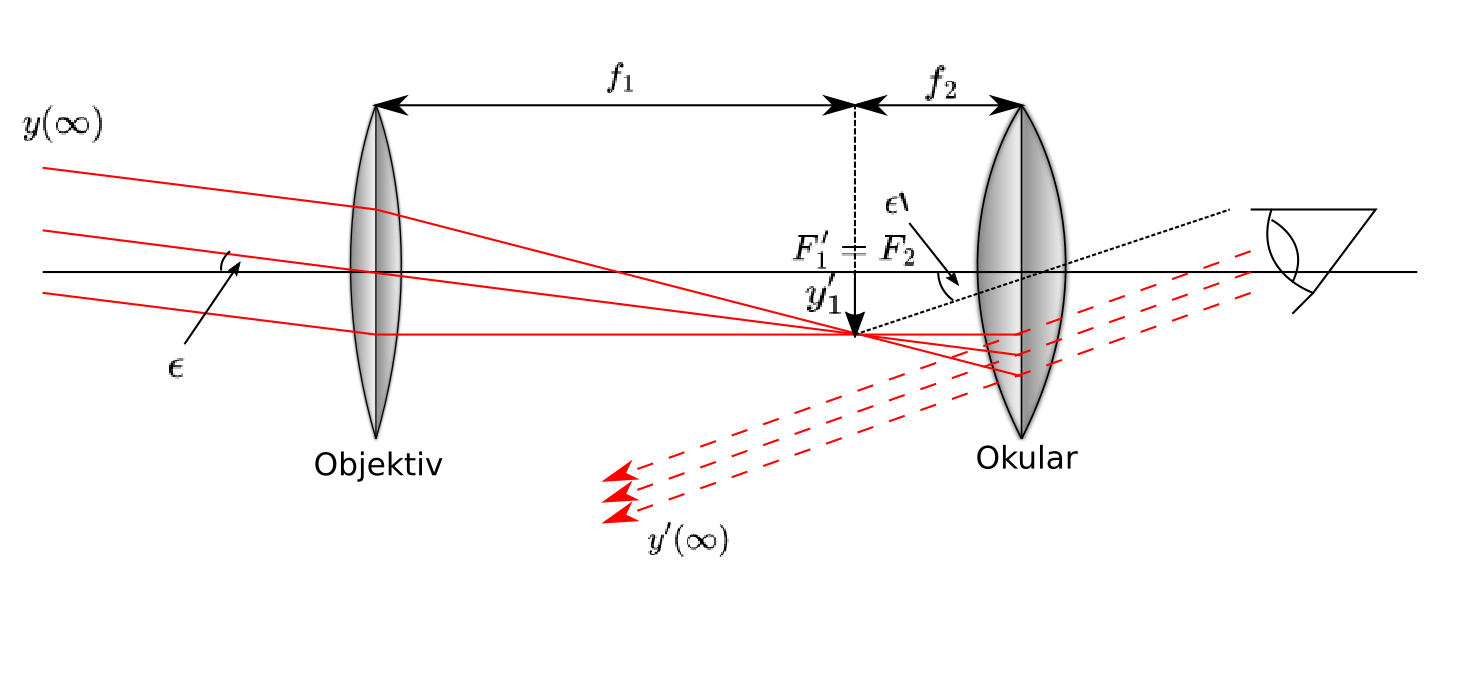
\includegraphics[scale=0.8]{Geometrische_Optik/Protokoll/fig/Kepplerfernrohr.png}
    \caption{Kepplerfernrohr}
    \label{fig:Kepplerfernrohr}
\end{figure}

\begin{figure}
    \centering
    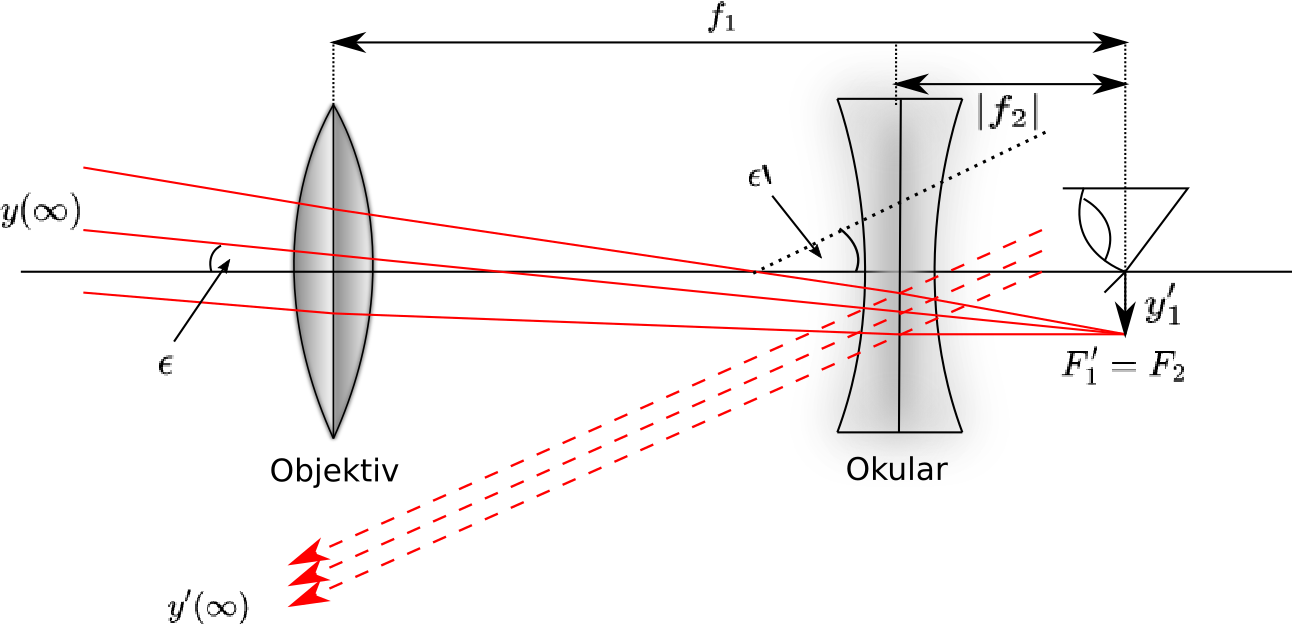
\includegraphics[scale=0.8]{Geometrische_Optik/Protokoll/fig/Galileofernrohr.png}
    \caption{Galileofernrohr}
    \label{fig:Galileofernrohr}
\end{figure}

\section{Bau eines Projektionsapparats}

\begin{figure}
    \centering
    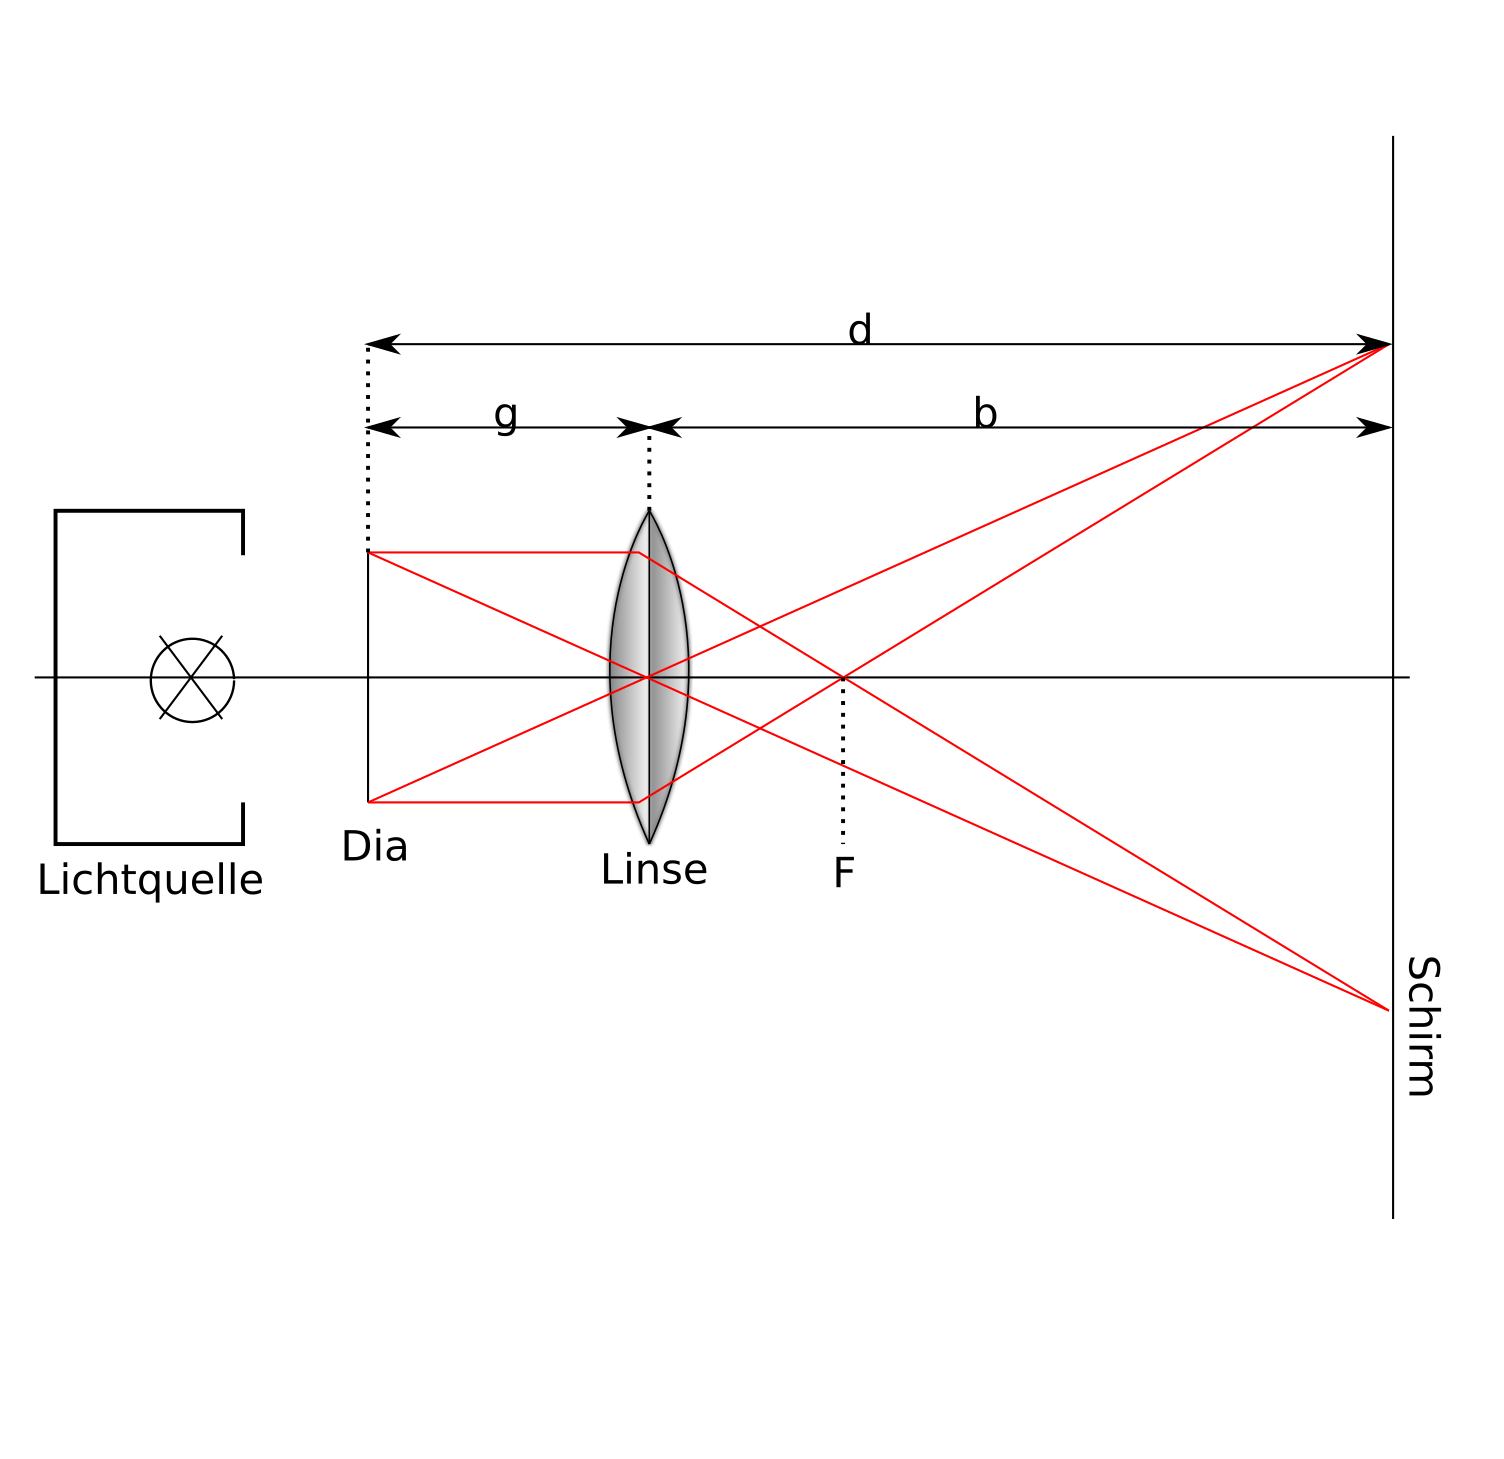
\includegraphics[scale=0.8]{Geometrische_Optik/Protokoll/fig/Diaprojektor.png}
    \caption{Diaprojektor}
    \label{fig:Diaprojektor}
\end{figure}

\section{Bau eines Mikroskops}

\begin{figure}
    \centering
    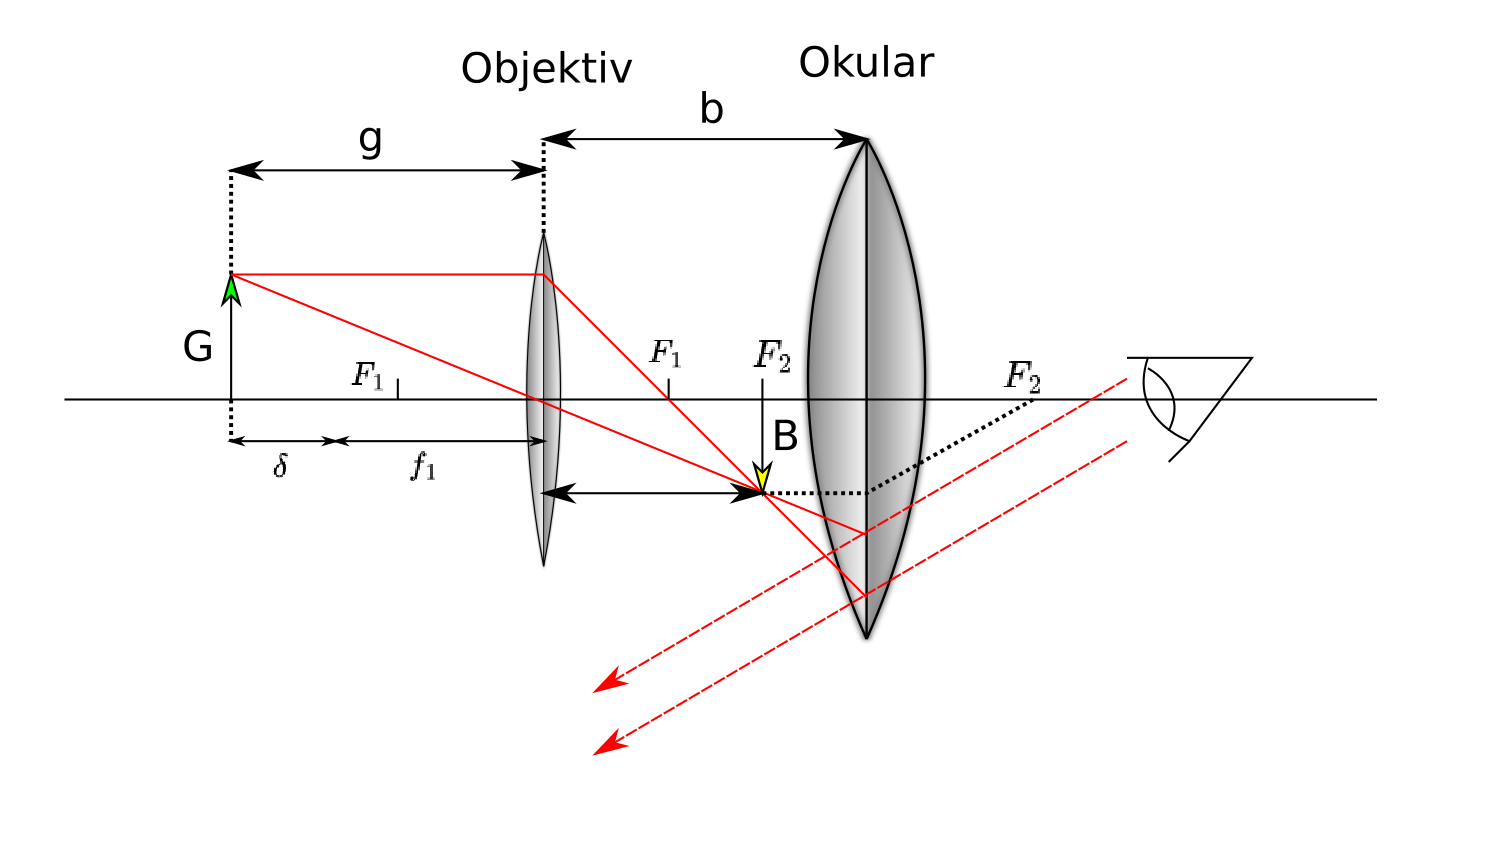
\includegraphics[scale=0.8]{Geometrische_Optik/Protokoll/fig/Mikroskop.png}
    \caption{Mikroskop}
    \label{fig:Mikroskop}
\end{figure}